
%%%%%%%%%%%%%%%%%%%%%%%%%%%%%%%%%%%%%%%%%%%%%%%%%%%%%%%%%%%%%%%%%%%%%%%%
% Evaluation
%%%%%%%%%%%%%%%%%%%%%%%%%%%%%%%%%%%%%%%%%%%%%%%%%%%%%%%%%%%%%%%%%%%%%%%%
\section{Experimental Study}
\label{sec:evaluation}

%-------plots------
\begin{table*}[!htbp]\footnotesize
\scriptsize
\begin{tabular}{lll}

%HOSP 
\begin{tikzpicture}
    \begin{axis}[
        legend pos=outer north east,        
        title=(a) \textsc{hosp} Data Cleaning for 90k,
        xlabel=noise,
        ylabel=F1, ]

         \addplot[mark=diamond] table[x=NOISE, y=CFDF1] {data/hosp-evaluation-90-datasize.tsv};
         \addplot table[x=NOISE, y=MDF1] {data/hosp-evaluation-90-datasize.tsv};
         \addplot table[x=NOISE, y=CFDMDF1] {data/hosp-evaluation-90-datasize.tsv};

        \legend{$cfd$,$md$,$cfd+md$},

    \end{axis}
\end{tikzpicture}
    &  
    

    \begin{tikzpicture}
%\selectcolormodel{gray}
   \begin{axis}[
       legend pos=outer north east,
       title=(b) \textsc{hosp} Data Cleaning for noise 10\%,
       xlabel=data size in k,
       ylabel=F1, ]

         \addplot[mark=diamond] table[x=DATASIZE, y=CFDF1] {data/hosp-evaluation-10-noise.tsv};
         \addplot table[x=DATASIZE, y=MDF1] {data/hosp-evaluation-10-noise.tsv};
         \addplot table[x=DATASIZE, y=CFDMDF1] {data/hosp-evaluation-10-noise.tsv};

       \legend{$cfd$,$md$,$cfd+md$},

   \end{axis}
\end{tikzpicture}
&
\begin{tikzpicture}
%\selectcolormodel{gray}
   \begin{axis}[
       legend pos=outer north east,
       title=(c) Runtime for \textsc{hosp} Data Cleaning,
       xlabel=data size in k,
       ylabel=seconds, ]

         \addplot[mark=diamond] table[x=DATASIZE, y=TIME] {data/hosp-evaluation-2-noise.tsv};
         \addplot table[x=DATASIZE, y=TIME] {data/hosp-evaluation-4-noise.tsv};
         \addplot table[x=DATASIZE, y=TIME] {data/hosp-evaluation-6-noise.tsv};
         \addplot table[x=DATASIZE, y=TIME] {data/hosp-evaluation-8-noise.tsv};
         \addplot table[x=DATASIZE, y=TIME] {data/hosp-evaluation-10-noise.tsv};

       \legend{$noise 2$,$noise 4$,$noise 6$,$noise 8$,$noise 10$},

   \end{axis} 
   \end{tikzpicture}

 \\
%TPC-H results

\begin{tikzpicture}
%\selectcolormodel{gray}
  \begin{axis}[
      legend pos=outer north east,
      title=(d) \textsc{tpc-h} Data Cleaning for 20000k,
      xlabel=noise,
      ylabel=F1, ]

         \addplot[mark=diamond] table[x=NOISE, y=CFDF1] {data/tpch-evaluation-20000-datasize.tsv};
         \addplot table[x=NOISE, y=MDF1] {data/tpch-evaluation-20000-datasize.tsv};
         \addplot table[x=NOISE, y=CFDMDF1] {data/tpch-evaluation-20000-datasize.tsv};

      \legend{$cfd$,$md$,$cfd+md$},

  \end{axis}
\end{tikzpicture}

& \begin{tikzpicture}
%\selectcolormodel{gray}
  \begin{axis}[
      legend pos=outer north east,
      title=(e) \textsc{tpc-h} Data Cleaning for noise 2\%,
      xlabel=data size,
      ylabel=F1, ]

         \addplot[mark=diamond] table[x=DATASIZE, y=CFDF1] {data/tpch-evaluation-2-noise.tsv};
         \addplot table[x=DATASIZE, y=MDF1] {data/tpch-evaluation-2-noise.tsv};
         \addplot table[x=DATASIZE, y=CFDMDF1] {data/tpch-evaluation-2-noise.tsv};

      \legend{$cfd$,$md$,$cfd+md$},

  \end{axis}
\end{tikzpicture} & 

\begin{tikzpicture}
%\selectcolormodel{gray}
  \begin{axis}[
      legend pos=outer north east,
      title=(f) Runtime for TPCH Data Cleaning,
      xlabel=data size,
      ylabel=seconds, ]

         \addplot[mark=diamond] table[x=DATASIZE, y=TIME] {data/tpch-evaluation-2-noise.tsv};
         \addplot table[x=DATASIZE, y=TIME] {data/tpch-evaluation-4-noise.tsv};
         \addplot table[x=DATASIZE, y=TIME] {data/tpch-evaluation-6-noise.tsv};
         \addplot table[x=DATASIZE, y=TIME] {data/tpch-evaluation-8-noise.tsv};
         \addplot table[x=DATASIZE, y=TIME] {data/tpch-evaluation-10-noise.tsv};

      \legend{$noise 2$,$noise 4$,$noise 6$,$noise 8$,$noise 10$},

  \end{axis}
\end{tikzpicture}
\end{tabular}
\caption{\label{tab:plots} Evaluation of the data repair method based on Markov logic applied on the ~\textsc{hosp} and~\textsc{tpc-h} data sets. (a)-(c) Data repair on \textsc{hosp} with an extended Markov logic method. (d)-(f) Experimantal study of the Markov logic data cleaning on synthetic data set \textsc{tpc-h}.}
\end{table*}


\begin{table}[t]\footnotesize
\scriptsize
\centering
\begin{tabular}{@{}ccccc@{}}
\toprule
{\bf experiment}       & {\bf \begin{tabular}[c]{@{}c@{}}numer \\ of tuples\end{tabular}} & {\bf \begin{tabular}[c]{@{}c@{}}evidence\\ atoms\end{tabular}} & {\bf \begin{tabular}[c]{@{}c@{}}number\\ of formulas\end{tabular}}  & {\bf \begin{tabular}[c]{@{}c@{}}runtime\\ (sec)\end{tabular}} \\ 
%\midrule
%                     & 63K                                                              & 266K                                                        & 21                                                                                                                                        & 2551                                                           \\
%{\bf \textsc{base}}           & 83K                                                              & 446K                                                        & 21                                                                                                                                        & 5128                                                           \\
%\multicolumn{1}{l}{} & 143K                                                             & 1286K                                                        & 21                                                                                                                                        & 12576                                                          \\
\midrule
                     & 63K                                                              & 266K                                                        & 21                                                                                                                                        & 242                                                           \\
{\bf \textsc{hosp}}           & 83K                                                              & 446K                                                        & 21                                                                                                                                        & 477                                                           \\
\multicolumn{1}{l}{} & 143K                                                             & 1286K                                                        & 21                                                                                                                                        & 1107                                                          \\ \midrule
\multicolumn{1}{l}{} & 20K                                                              & 210K                                                        & 15                                                                                                                                        & 41                                                            \\
{\bf \textsc{tpc-h}}           & 40K                                                              & 419K                                                        & 15                                                                                                                                        & 131                                                           \\
\multicolumn{1}{l}{} & 100K                                                             & 1055K                                                        & 15                                                                                                                                        & 732                                                           \\ \bottomrule
\end{tabular}
\caption{\label{tab:runtime} Scalability of the data cleaning for \textsc{tpc-h} and \textsc{hosp} data sets (with fixed noise 4\%). }
\end{table}


\begin{table*}[t]\footnotesize
\scriptsize
\centering
\begin{tabular}{@{}llll@{}}
\toprule
& \multicolumn{1}{c}{\textsc{hosp}}  & \multicolumn{1}{c}{\textsc{tpc-h}}  & \multicolumn{1}{c}{\textsc{msag}}  \\ \midrule
\begin{tabular}[c]{@{}l@{}}
 observed\\ predicates
\end{tabular} 
& 
\begin{tabular}[c]{@{}l@{}}
\textsf{providerNr/\textsc{hosp}}(hid, pn)\\ 
\textsf{hospitalName/\textsc{hosp}}(hid, n)\\ 
\textsf{address/\textsc{hosp}}(hid, add)\\ 
\textsf{city/\textsc{hosp}}(hid, c)\\ 
\textsf{state/\textsc{hosp}}(hid, st)\\ 
\textsf{zipCode/\textsc{hosp}}(hid, code)\\ 
\textsf{countryName/\textsc{hosp}}(hid, country)\\ 
\textsf{phoneNumber/\textsc{hosp}}(hid, numb)\\ 
\textsf{condition/\textsc{hosp}}(hid, cond)\\ 
\textsf{measureCode/\textsc{hosp}}(hid, mcode)\\ 
\textsf{measureName/\textsc{hosp}}(hid, mname)\\ 
\textsf{score/\textsc{hosp}}(hid, score)\\ 
\textsf{zip/\textsc{zipcode}}(zid, code)\\ 
\textsf{state/\textsc{zipcode}}(zid, st)
\end{tabular}                       
& 
\begin{tabular}[c]{@{}l@{}}
\textsf{custKey}(id, key)\\ 
\textsf{name}(id, n)\\ 
\textsf{addr}(id, add)\\ 
\textsf{natKey}(id, nkey)\\ 
\textsf{phone}(id, ph)\\ 
\textsf{acc}(id, a)\\ 
\textsf{mrkt}(id, m)\\ 
\textsf{orderKey}(id, okey)\\ 
\textsf{orderStatus}(id, st)\\ 
\textsf{totalPrice}(id, p)\\ 
\textsf{orderDate}(id, d)\\ 
\textsf{orderPriority}(id, pr) \\ 
\textsf{clerk}(id, c)
\end{tabular} 
& 
\begin{tabular}[c]{@{}l@{}}
\textsf{publishYear}(paperid, pubyear)\\
\textsf{author}(paperid, authorid)\\
\textsf{affiliation}(paperid, affilid)\\
\textsf{inRange}(pubyear, pubyear)\\
\textsf{originAffiliationName}(affilid, oname)\\
\textsf{normalAffiliationName}(affilid, nname)
\end{tabular}
\\ \midrule % now hidden predicates
\begin{tabular}[c]{@{}l@{}}
hidden \\ predicates
\end{tabular}  
& \begin{tabular}[c]{@{}l@{}}
  \textsf{equal-HospitalName/\textsc{hosp}}(hid, n, hid, n)\\ 
  \textsf{equal-Address/\textsc{hosp}}(hid, add, hid, add)\\ 
  \textsf{equal-City/\textsc{hosp}}(hid, c, hid, c)\\ 
  \textsf{equal-State/\textsc{hosp}}(hid, st, hid, st)\\ 
  \textsf{equal-ZipCode/\textsc{hosp}}(hid, code, hid, code)\\ 
  \textsf{equal-CountryName/\textsc{hosp}}(hid, ctr, hid, ctr)\\ 
  \textsf{equal-PhoneNumber/\textsc{hosp}}(hid, nr, hid, nr)\\ 
  \textsf{equal-MeasureName/\textsc{hosp}}(hid, mn, hid, mn)\\ 
  \textsf{equal-Condition/\textsc{hosp}}(hid, cond, hid, cond)\\ 
  \textsf{\textsc{hosp}/match-State/\textsc{ZipCode}}(hid, zid)\\ 
  \textsf{\textsc{hosp}/match-ZipCode/\textsc{ZipCode}}(hid, code)
\end{tabular} 
& 
\begin{tabular}[c]{@{}l@{}}
 \textsf{equal-Names}(id, n, id, n)\\ 
 \textsf{equal-Addr}(id, add, id, add)\\ 
 \textsf{equal-Natkey}(id, nkey, id, nkey)\\ 
 \textsf{equal-Phone}(id, ph, id, ph)\\ 
 \textsf{equal-Acc}(id, a, id, a)\\ 
 \textsf{equal-Mrkt}(id, m, id, m)\\ 
 \textsf{match-Phone}(id, id)\\ 
 \textsf{match-Addr}(id, id)
\end{tabular} 
& 
\begin{tabular}[c]{@{}l@{}}
\textsf{equal-Affiliation}(paperid, paperid)\\
\textsf{equal-OriginNames}(oname, oname)\\
\textsf{equal-OriginNamesByPaperId}(paperid, paperid)\\
\textsf{equal-NormalNames}(nname, nname)\\
\textsf{equal-NormalNamesByPaperId}(paperid, paperid)\\
\textsf{missingOriginName}(paperid, oname)
\end{tabular}\\ \bottomrule
\end{tabular}
\caption{\label{tab:predicates} Markov logic predicates used in data quality rules.}
\end{table*}


We now evaluate our method through an experimental study in which we execute our method on a 
well-known data sets used for evaluating another data cleaning systems. Each of the data sets suffers from different data quality issues such as duplicates, inconsistency or missing values. To evaluate the effectiveness of our method we asses the accuracy and the scalability of proposed data cleaning with Markov logic.% We provide a quality assessment and runtime evaluation for each of the datasets. 

\subsection{Experimental Setting} 
We conducted our experiments on a real-life and synthetic data sets, which were also used by previous work to investigate data cleaning approaches. We also distinguish between relational data formats and Web data. 
\todo[inline]{make our data public}

\textbf{\textsc{hosp}}. The \textsc{hosp} data set is taken from US Department of Health $\&$ Human Services\footnote{http://www.medicare.gov/hospitalcompare/Data/Data-Download.html}. This data set comprises 9 attributes: \textsf{addr}, \textsf{city}, \textsf{cond}, \textsf{country}, \textsf{hospname}, \textsf{measure}, \textsf{phone}, \textsf{state}, \textsf{zip}. 
We used 6 CDFs and one MD, which were manually designed. These data quality rules were generously provided to us by the researchers Dallachiesa, M. et al. from~\cite{Dallachiesa:2013:NCD:2463676.2465327}. One example of their rules is a CFD that states that if two tuples of \textsf{hosp} agree on attribute values for $\textsf{zip}$, then they should also agree on \textsf{country} and \textsf{state} attributes values. They define one MD that makes use of another table, namely US ZIP codes: ZIPCode\footnote{http://databases.about.com/od/access/a/zipcodedatabase.htm}. This additional data set contains $43K$ tuples with two attributes: \textsf{zip} and \textsf{state}. The MD defines that if two tuples from \textsf{hosp} and ZIPCode respectively possess the same zip code values, and the state values are distinct, then the state value from the ZIPCode table should be adopted. 

\textbf{\textsc{tpc-h}.} The \textsc{tpc-h}\footnote{http://www.tpc.org/tpch/} is well-known data set used in decision support benchmarks for databases. For our experiments we used two relations \textit{Customer} and \textit{Orders}, wich we joined in order to introduce duplications on the \textit{Customer} relations data. The resulted data set consists of 17 attributes of schema $T$: \textsf{c\_custkey}, \textsf{c\_name}, \textsf{c\_address},  \textsf{c\_nationkey}, \textsf{c\_phone}, \textsf{c\_acctbal},\\ \textsf{c\_mtksegment}, \textsf{c\_comment}, \textsf{o\_orderkey}, \textsf{o\_custkey},\\ \textsf{o\_orderstatus}, \textsf{o\_totalprice}, \textsf{o\_orderdate},\\ \textsf{o\_orderpriority}, \textsf{o\_clerk}, \textsf{o\_shippriority}, \textsf{o\_comment}. 

\textbf{Dirty Data.} The dirty data on relational data sets \textsc{hosp} and \textsc{tpc-h} is produced by introducing noise. There are several arts of noise our method is capable to deal with: missing values, errors from the active domain and typos. The initial data set is considered as being clean and therefore acting as a ground truth. We also manually assessed that the ground truth data set is consistent regarding the CFDs and MDs. Afterwards, we inserted noise to the data sets. We conducted our experiments on two data sets with a different noise rate ranging from $\mathsf{noi\%}$=2$\%$ to $\mathsf{noi\%}$=10$\%$, which were introduced into different data sets sizes ranging from 1k to 100k data points. The noise rate is a ratio of the number of erroneous values to the total number of values in the data set. Furthermore, we only introduced noise to the attributes which are involved in data quality rules.

\textbf{\textsc{microsoft academic graph (msag)}.} Data quality issues are massively present in the context of the Web due to integration of heterogeneous data from different sources. Thus, to asses our method on the Web data cleaning, we include a third data set - \textsc{microsoft academic graph (msag)}\footnote{http://research.microsoft.com/en-us/projects/mag/} \cite{msag2015}, which is a heterogeneous entity graph comprised of six types of entities that model the real-life academic relationships: field of study, author, institution, paper, venue, and conference instances. The raw data is obtained from different sources (academic publishers and web-pages indexed by Bing search engine) and organized as connected graph schema. For our experiments, we selected three entities from the whole graph, namely \textit{author}, \textit{organisation} and \textit{paper} entities. This part of \textsc{msag} is of interest because it reveals important characteristics of extracted web data, such as missing and inconsistent values. In particular, we discovered that there are inconsistencies in organisation names for the same author. Furthermore, a number of entries suffer from missing affiliation by an author. In order to model and run data cleaning on web (graph) data, we consider the attributes of the selected entities in \textsc{msag} presented in Table \ref{tab:msagattrs}. 
\begin{table}[t]\footnotesize
\scriptsize
\centering
\begin{tabular}{ccc}
\textbf{\textit{Paper}}         & \textbf{\textit{Author}}     & \textbf{\textit{Organisation}}      \\ \hline
\textsf{paper\_id}     & \textsf{author\_id} & \textsf{affiliation\_id}  \\
\textsf{publish\_year} &            & \textsf{origin\_name}     \\
              &            & \textsf{normalized\_name}\\ \hline
\end{tabular}
\caption{Entities \textbf{\textit{Paper}}, \textbf{\textit{Author}} and \textbf{\textit{Organisation}} and their attributes that have been used in experiments for Web data cleaning with Markov Logic.}
    \label{tab:msagattrs}
\end{table}

\textbf{Data Quality Issues.} To perform data cleaning experiments on web data we extracted a subset of entities instances, which were complete. Having this clean data we reproduced data quality issues that we observed in \textsc{msag}: namely missing values. In order to create gold standard to asses the data cleaning method we proceed in the following way: We removed one affiliation entry from each author if there were more than three publications made by the same affiliation. In this way we created a data set with missing \textsf{affiliation\_id}, \textsf{origin\_name} and \textsf{normalized\_name} attributes. In general, we obtained graph data where $37\%$ of all authors reveal one missing edge to theirs affiliation; $27\%$ are missing two edges for theirs institutions; $15\%$ - three edges. Almost $21\%$ suffers from missing more than three edges. 

\begin{figure}[t]
    \centering
    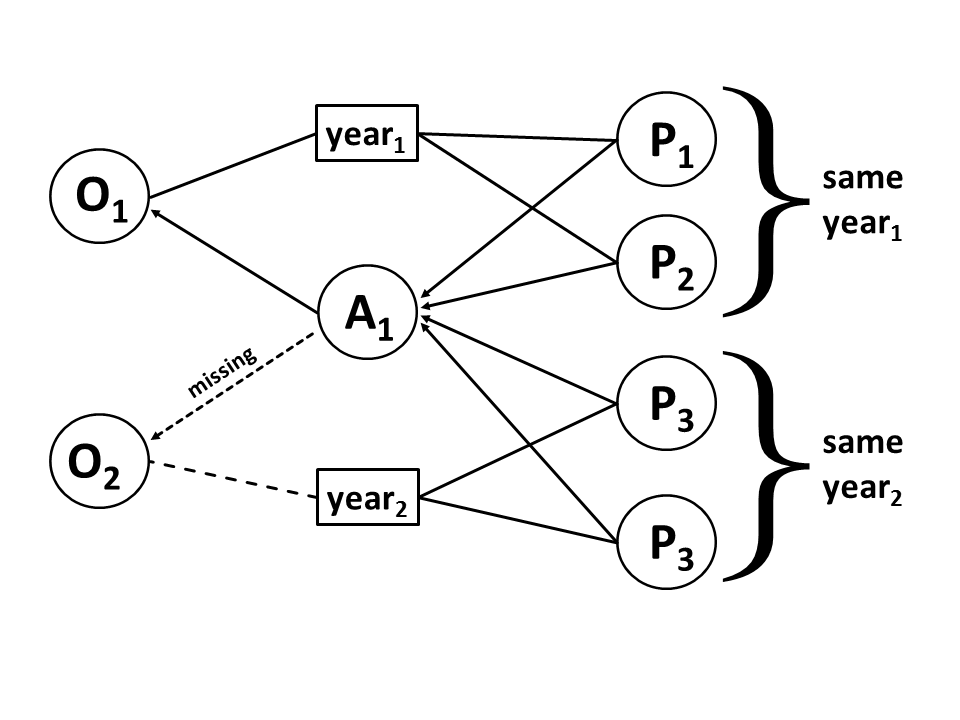
\includegraphics[width=0.25\textwidth, trim = 0mm 4mm 0mm 5mm, clip]{img/graph01.png}
    \caption{The part of the \textsc{msag} data set illustrating missing organisation value issue. Markov Logic affords to capture the following regularity that if two papers of the same author published in the same year, this is evidence that they were published by the author of the same organisation. Nodes notation: A - denotes \textit{Author} entity; O - \textit{Organisation} and P - \textit{Paper} entities. Missing edges are marked as dashed lines.}
    \label{fig:msagmissing}
\end{figure}

\textbf{Evaluation metrics.} We evaluate the effectiveness of our data cleaning method and consider hence two aspects: the accuracy and the scalability of the method. To assess the quality of the data cleaning framework on relational data, we use \textit{Precision ($P$)}, \textit{Recall ($R$)} and \textit{F-measure ($F_1$)}. We also acquired master data (also referred to as \textit{"gold standard"}), which is clean and correct. We use this master data to determine $true~positives (tp)$ - correctly selected by the method attribute values; $false~positives (fp)$- is a degree of false assignment of the attribute values that are selected to be corrected and $false~negatives (fn)$- correct attribute value, which were not found by our framework.

\begin{tabular}{ l l l }
$~P=\frac{tp}{tp+fp}~$ & $~R=\frac{tp}{tp+fn}~$ & $~F_1=\frac{2PR}{P+R}~$ \\
\end{tabular}

Therefore, precision is the ratio of true positives to all values found and recall is the ratio of true positives to the all correct values. We computed the $F_1$ measure, which is the harmonic mean of precision and recall.

The efficiency of our method we asses by running our experiments on data sets of different size ranging from 1k to 100k tuples each.

We leverage the state-of-the-art inference engine for Markov logic \textit{RockIt}, developed by Noessner J. et al.~\cite{NoessnerNS13} for Markov logic modeling and performing statistical inference. All results in our experiments were achieved by applying MAP inference method for Statistical Relational Learning by performing on Linux machine with an Intel 3.4GHz 4 Cores CPU 16GB RAM.


\subsection{Experimental Results} 
%\todo[inline]{For each experiment follow the structure: 
%1. Corresponding Contribution
%2. Experimental Setup (Dataset; Method)
%3. Results (Describe plots, measures etc.)
%4. Explanation (Why we have such results) and Relation to Contribution
%}

\textbf{Exp-1: Usability in modeling of data cleaning rules.}

%Big table containing all the rules and formulas:
\begin{table*}[t]\footnotesize
\scriptsize
\centering

\begin{tabular}{cll}
\textbf{\textit{Data Set}}               & \multicolumn{1}{c}{\textbf{\textit{Data Cleaning Rules}}}              & \multicolumn{1}{c}{\textbf{\textit{Markov Logic Formulae}}} \\ \hline
%hosp
\multirow{2}{*}{\textsc{hosp}}  & %hosp dq rules
                        \begin{tabular}[c]{@{}l@{}}
                        $\mathsf{cfd_1: \textsc{hosp}([\textsf{zip}] \rightarrow [\textsf{state, city}], t1=(\_ \parallel \_, \_))}$\\
                        $\mathsf{cfd_2: \textsc{hosp}([\textsf{phone}] \rightarrow [\textsf{addr, zip,state, city}],t2=(\_ \parallel \_,\_,\_,\_))}$
                        \end{tabular}                   
                        & %hosp markov logic cfd
                        \begin{tabular}[c]{@{}l@{}}
                        $\mathsf{w_1: \textsf{zip}(id1, code)~\wedge~\textsf{zip}(id2, code)~\wedge \textsf{state}(id1, s1)~\wedge~\textsf{state}(id2, s2)~}$ \\
                        $\mathsf{~~~~~~~~\wedge!\textsf{state}(id1, s2)~\wedge~!\textsf{state}(id2, s1)~\Rightarrow \textsf{equal-state}(id1, s1, id2, s2)}$\\
                        %second cfd:
                        $\mathsf{w_2: \textsf{zip}(id1, code)~\wedge~\textsf{zip}(id2, code)~\wedge \textsf{city}(id1, c1)~\wedge~\textsf{city}(id2, c2)~}$ \\
                        $\mathsf{~~~~~~~~\wedge!\textsf{city}(id1, c2)~\wedge~!\textsf{city}(id2, c1)~\Rightarrow \textsf{equal-city}(id1, c1, id2, c2)}$
                        \end{tabular}                 \\ 
                       & %hosp md rule
                         \begin{tabular}[c]{@{}l@{}}
                        $\mathsf{md_1: \textsc{hosp}[\textsf{zip}]=\textsc{zipcode}[\textsf{zip}]\wedge \textsc{hosp}[\textsf{state}]\neq \textsc{zipcode}[\textsf{state}]}$\\
                        $\mathsf{~~~~~~~~~~~~~~\rightarrow\textsc{hosp}[\textsf{state}]\rightleftharpoons \textsc{zipcode}[\textsf{state}]} $
                        \end{tabular}                 
                       & %hosp markov logic md
                       \begin{tabular}[c]{@{}l@{}}
                        $ todo $
                       \end{tabular}                  
                       \\ \hline

%tpc-h
\multirow{2}{*}{\textsc{tpc-h}} & %tpc-h fds
                        \begin{tabular}[c]{@{}l@{}}
                        $\mathsf{cfd_1: \textsc{t}([\textsf{c\_custkey}] \rightarrow [\textsf{c\_name,c\_address}],t1=(\_ \parallel \_, \_))} $
                        \end{tabular}                   
                        &%tpc-h mlogic fds
                         \begin{tabular}[c]{@{}l@{}}
                        $ todo $
                        \end{tabular}                    
                         \\  
                       & %tpch md rules
                       \begin{tabular}[c]{@{}l@{}}
                        $\mathsf{md_1: \textsc{t}[\textsf{c\_address}]=\textsc{t}[\textsf{c\_address}] \rightarrow \textsc{t}[\textsf{c\_phone}]\rightleftharpoons \textsc{t}[\textsf{c\_phone}]}$\\ 
                        $\mathsf{md_2: \textsc{t}[\textsf{c\_name}]=\textsc{t}[\textsf{c\_name}] \rightarrow \textsc{t}[\textsf{c\_address}]\rightleftharpoons \textsc{t}[\textsf{c\_address}]} $

                        \end{tabular}                  
                       & %tpch md markov logic
                       \begin{tabular}[c]{@{}l@{}}
                        $ todo $
                        \end{tabular}                     
                       \\ \hline
%msag
\multirow{3}{*}{\textsc{msag}}  & % msag fd
                                \begin{tabular}[c]{@{}l@{}}
                                $\mathsf{cfd_1: \textsc{m}([\textsf{author\_id, year}] \rightarrow [\textsf{affiliation\_id}],t1=(\_,\_ \parallel \_))} $\\
                                $\mathsf{cfd_2: \textsc{m}([\textsf{affiliation\_id}] \rightarrow [\textsf{origin\_name}],t2=(\_ \parallel \_))} $
                                \end{tabular}                   
                                & %msag markov logic fd
                                \begin{tabular}[c]{@{}l@{}}
                                $todo $
                                \end{tabular}                   
                                \\  
                                & % msag extended fd
                                \begin{tabular}[c]{@{}l@{}}
                                 $\mathsf{eCfd_1: \textsc{m}([\textsf{author\_id, year}] \rightarrow [\textsf{affiliation\_id}],t1=(\_, diff(\_)\leq 2 \parallel \_))} $   
                                \end{tabular}             
                                & % msag markov logic 
                                \begin{tabular}[c]{@{}l@{}}
                                $ todo $
                                \end{tabular}  
                                \\
                                &%additional predicates for msag
                                %nothing here
                                & Equality axioms:
                                \begin{tabular}[c]{@{}l@{}}
                                $symmetry$\\
                                $transitivity$
                                \end{tabular}  

                                \\ \hline
\end{tabular}
\caption{Usability in modeling of data cleaning rules as Markov Logic programs.}
\label{tab:rulesformulas}
\end{table*}

In this part of experiments we show the feasibility of translating the data quality rules into Markov logic applied on noisy data.This part of experiments we conducted on all three data sets described above. 

\textbf{\textsc{hosp} Quality Rules}. In our data cleaning method for the \textsc{hosp} data we use 6 manually designed CDFs and one MD, which resulted in 15 normalized CFDs. One MD rule is transformed into 2 formulas. All data cleaning rules are positive. In the current experiments we have not modeled negative data cleaning rules, although such rules can be trivially defined within the Markov logic framework. Finally, all interleaved rules were translated into 21 Markov logic formulas. In the Table \ref{tab:rulesformulas} we provide an example of the above specified data quality rules (not normalized CFD), which were defined on pair of tuples. The MD rule is specified on a two relations. Markov logic predicates used for data quality formulae are shown in Table~\ref{tab:predicates}. After transforming the 100k \textsc{hosp} tuples into Markov logic grounded atoms, the resulting data comprises 1.3Mio evidence atoms, which are then used for the inference. We also empirically observed that extending the data quality rules set for for some additional conditions reduces the search space and therefore converges much faster than \textit{"pure"} model. This means that each first order logic formula, which represent the RHS of the normalized data quality rule $\mathsf{\textsf{attr}(id1, v1)~\wedge~\textsf{attr}(id2, v2)}$ becomes an inverse part $\mathsf{!\textsf{attr}(id1, v2)~\wedge~!\textsf{attr}(id2, v1)}$. This additional part denotes that we consider only tuples with different values. Here the normalized CFD rules are being compiled as demonstrated in the Table \ref{tab:rulesformulas}. 

\textbf{\textsc{tpc-h} Quality Rules}. For this data set 9 CFDs and 3 MDs have been written. One example of the rules is a CFD that states if two tuples agree on \textsf{c\_custkey}, then they should agree on \textsf{c\_name} and \textsf{c\_address} attributes. For this part of experiments, MDs are designed on the same schema \textsc{tpc-h} \textsf{(T, T)}. These MDs state that for any pair of tuples $(t_1,t_2)$ if the LHS is similar, then the attribute values on the RHS should be identified. In the Table \ref{tab:rulesformulas} we provide an except of the data quality rules we created for \textsc{tpc-h}.
%//addr | phone : for two similar addreses the phone numbers should be same
%//name | addr : for two similar names the addreses should be same
Markov logic predicates used for data quality rules are shown in Table~\ref{tab:predicates}. After transforming the 100k \textsc{tpc-h} tuples into Markov logic grounded atoms, the resulting data comprises 1 Mio evidence atoms, which are then used for the inference.

\textbf{\textsc{msag} Quality Rules}.  
%\anno{explain core rules and adding general knowledge to the msag data cleaning.}
%\todo[inline]{MSAG: DQ rules for graph/Web data}
Due to the graph nature of the \textsc{msag} data (see Figure \ref{fig:msagmissing}) we developed data quality rules, which are based on CFDs, \textit{extended} CFDs \cite{Chen2009extended} and equality axioms, such as \textit{symmetry} and \textit{transitivity}. For the \textit{Paper}-\textit{Author}-\textit{Organisation} subgraph we defined two CFDs, one extended CFD and 8 additional rules that comprises equality axioms for hidden predicates. Considering the semantical meaning of the data, we profit from the ability to add supporting knowledge into data cleaning process. For example, having the CFD$\mathsf{\textsc{m}([\textsf{author\_id, year}] \rightarrow [\textsf{affiliation\_id}],t1=(\_,\_ \parallel \_))} $  allows us to capture all missing affiliation by the same author, what published in the same year. In real life we know that in academia an average contract lasts around 2-3 years. Therefore by incorporating this knowledge in form of a predicate $\mathsf{\textsf{inRange}(year, year)}$ we will extend our search range. Additionally, by combining with equality axioms, we enable capturing more missing values. For example, the hard rule $\mathsf{\textsf{equal-Affiliation}(id_1, id_2) ~\wedge~ \textsf{equal-Affiliation}(id_2, id_3) \Rightarrow  \textsf{equal-Affiliation}(id_1, id_3)}$ denotes transitive relationship between three different entities \textit{Organisation}. In total, Markov Logic program consists then from 21 lines of code.

In general, this part of our experimental study demonstrated that the expressiveness of Markov Logic affords us to model data cleaning rules in a convenient manner. Obviously, Markov Logic is data format independent, which facilitates data cleaning on different data formats as provided on relational and graph data formats. Direct translation data cleaning rules into first-order logic and therefore Markov Logic formulae simplifies the process of writing data cleaning routines. 

%%%%%%%%%%%
\textbf{Exp-2: Holistic data cleaning: Deduplication and Accuracy.} In this part of experiment we want to show that capturing the data issues interaction  positively influences the overall result in data cleaning. In particular, we are studying the connection between deduplication and improving data accuracy.

We evaluated the accuracy of our method applied on different noise rate and different data set size. For this part of experiment we introduced noise by adding either typos or replacing values of attributes (active domain errors). In our experiments we do not distinguish these two art of errors. As shown in Table~\ref{tab:plots} results of using Markov logic programs for data cleaning is demonstrated by (a)-(c) for \textsc{hosp} and (d)-(f) for \textsc{tpc-h}. Here we could achieve excellent results in errors identifying. We compare results of separate execution of CDFs and MDs. After that we ran our experiments by combining CFDs and MDs. Because CFDs and MDs are modeled together in a single model for identifying dirty data, they are treated jointly and therefore we do not have any influence on order of the data quality rules execution. The provided results clearly demonstrate that joint execution improves the overall result. In particular, the low $F_1$ score of MDs can be explained by the low precision and high recall. Although, by adding CFDs to MDs the overall $F_1$ score improves. 

The counterintuitive improvement of the $F_1$ values while increasing noise in Table~\ref{tab:plots} (a) and (d) can be explained by the \textit{Cutting Plane Inference} \cite{riedel08improving} behavior. For (almost perfect) data with less noise the algorithm runs less time and converges fast by finding (approximately) maximal objective score. This obviously results in detecting less data violations. Considering the runtime in Table~\ref{tab:plots} (c) and (f), we recognise that with increasing noise the underlying solver calculates solution until the maximum number of iterations are reached. Therefore, more data quality rules violations are encountered.    

This experiment tells us that the joint modeling and joint inference on detection data issues improves results achieved by running single data quality rules.

\textbf{Exp-3: Holistic data cleaning: Missing Value and Consistency Issues Interaction}
\pgfplotsset{small,  compat=1.5}
\begin{table*}[t]\footnotesize
\scriptsize
\centering
\begin{tabular}[t]{ll} %\hline
 
 \begin{tikzpicture}[baseline=0]
  %\begin{axis}[title=(a),
  %    xlabel=Recall,
  %    ylabel=$F_1$, ]
  %    \addplot+[only marks,mark=x] table[x=RECALL, y=F1] {data/msag-interpolated.tsv};
  %\end{axis}
    \begin{axis}[
      legend pos=outer north east,
      title=(a),
      xlabel=Recall,
      ylabel=F1, 
      legend entries={$1-2~missing~edges$,$3-4~missing~edges$,$more~than5$}, ]
         \addplot[ scatter,
                   only marks,
                   point meta=explicit symbolic,
                   scatter/classes={
                   a={mark=x,blue},%
                   b={mark=triangle,red},%
                   c={mark=o,draw=black}},] 
          table[x=RECALL, y=F1, meta=MARK] {data/msag-marked.tsv};
  \end{axis}
\end{tikzpicture}
&
 
 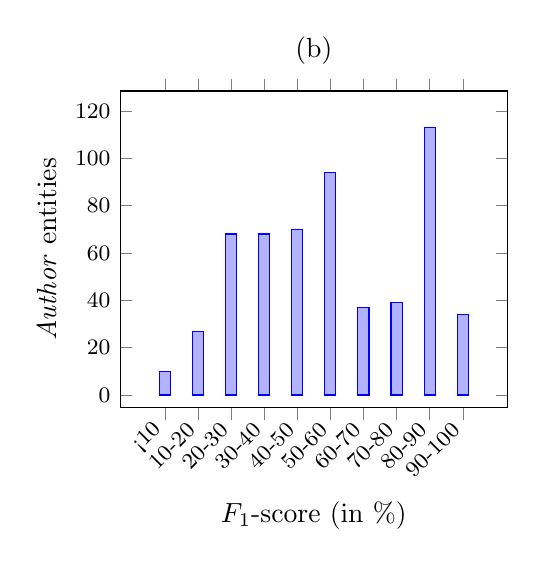
\begin{tikzpicture}[baseline=0]
        \begin{axis}[
        ybar,
        enlargelimits=0.15,
              %legend style={at={(0.5,-0.15)}, anchor=north,legend columns=-1},
        bar width=4,
        ylabel={\textit{Author} entities},
        xlabel={$F_1$-score (in \%)},
        title=(b),
        symbolic x coords={<10, 10-20, 20-30, 30-40, 40-50, 50-60, 60-70, 70-80, 80-90, 90-100},
        xtick=data,
        nodes near coords align={vertical},
        x tick label style={rotate=45,anchor=east},
        ]
        \addplot coordinates {(<10,10)
                              (10-20,27)
                              (20-30,68)
                              (30-40,68)
                              (40-50,70)
                              (50-60,94)
                              (60-70,37)
                              (70-80,39)
                              (80-90,113)
                              (90-100,34)};
        \end{axis}
      \end{tikzpicture}


 \\ %\hline
\end{tabular}
\caption{(a) \textsc{msag} cleaning: Recall and F1 values; (b) \textsc{msag} Experiments} 
\label{tab:msag}
\end{table*}

In the following experiment we studied the efficiency of the data cleaning on Web data by leveraging the connection between information completeness and data consistency. Meaning that to repair the attributes of an entity they should not be missing and on the other hand, for information completeness the data should be consistent. The initial size of the \textsc{msag} subgraph \textit{Paper}-\textit{Author}-\textit{Organisation} is about 30GB and certainly not tractable to run the inference on whole data. Therefore, in this experiment we partitioned our data by running inference for each author in separate. In this way we obtained subgraphs for each \textit{Author}-entity with number of \textit{Paper}-\textit{Author} edges beginning from 10. For this experiment we randomly selected 600 \textit{Author}-entities and Table \ref{tab:msag} (a) and (b) shows the accuracy of our approach on the sample of \textsc{msag} data set. The result shows the following: The method demonstrates overall $F_1$ score greater than $50\%$ and recall greater than $78\%$ for \textit{Author}-entities with one to two missing edges. Beginning from three missing edges we still are able to achieve a good recall, though the precision (and therefore $F_1$ score) drops. We explain this because our approach selects more false positives with increasing number of missing values. This experiment tells us that applying on Web data, our method can still produce good results, yet extending data cleaning rules with domain specific information should be studied further in order to reduce false positives values in data repair.

\textbf{Exp-4: Rules Execution Order}
%\todo[inline]{Execution order experiment description:  Dataset, method, results... Handling deduplication and accuaracy issues interaction}
The aim of this experiment is to study different orders of data cleaning rules execution. In particular, we aim to support our hypotheses that specifying the optimal order of rules execution is hardly achievable \cite{Dallachiesa:2013:NCD:2463676.2465327}, therefore leveraging joint inference for the simultaneous rules execution shall overtake the specification of the optimal order of rules execution. We run our Markov Logic program on \textsc{hosp} data set with $90k$ tuples by noise ranging from $2\%$ to $10\%$. This experiment consists of three parts: First, we run MD rule and then CFD and the overall performance is worst. This obviously corresponds to the previous Experiment-2 about joint modeling data cleaning rules (see also Table Table~\ref{tab:plots} (a)). The MD rule performs poor than CFD. Second, we changed the sequence of execution by running CFD first and then MD rule. This slightly improves $F_1$ scores because initially CFD is able to detect more violations. Finally, we performed the joint execution of CFD and MD rules, which confirms our hypotheses that multiple data cleaning rules should be executed simultaneously. The result is shown in Figure \ref{fig:orderexec}. This experiment demonstrates that the order of execution matters and different order produces distinct results.

%\pgfplotsset{small,  compat=1.5}

\begin{figure}
\centering
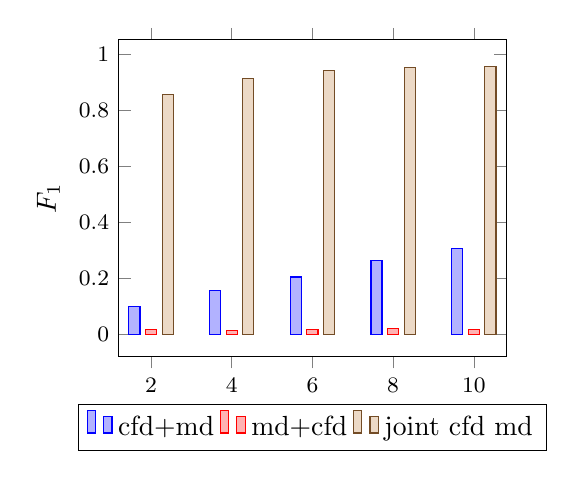
\begin{tikzpicture} 
\begin{axis}[
ybar,
enlargelimits=0.1,
legend style={at={(0.5,-0.15)}, anchor=north,legend columns=-1},
bar width=4,
ylabel={$F_1$},
symbolic x coords={2,4,6,8,10},
xtick=data,
nodes near coords align={vertical},
]
\addplot coordinates {(2, 0.1) (4, 0.1552) (6, 0.2039) (8, 0.2625) (10, 0.3048)};
\addplot coordinates {(2, 0.0176) (4, 0.0139) (6, 0.0173) (8, 0.0214) (10, 0.016)};
\addplot coordinates {(2, 0.8566) (4, 0.9114) (6, 0.9403) (8, 0.9512) (10, 0.9569)};

\legend{cfd+md,md+cfd,joint cfd md}

\end{axis}
\end{tikzpicture}
\caption{Order execution with Markov Logic} 
\label{fig:orderexec}
\end{figure}



\textbf{Exp-5: Efficiency.} To assess the efficiency of our method we studied the runtime of our method for different data size and noise rate. This is shown in Figure~\ref{tab:plots} (c) for \textsc{hosp} and (f) for \textsc{tpc-h} and in Table~\ref{tab:runtime}. This experiment tells us that our method is robust against noise, but adding more noise leads to higher runtime. By reducing the search space in Markov logic we were able to reduce the runtime by factor 10. Furthermore, the predicate-arity used in Markov logic formulas influences the runtime of data cleaning. Empirically, the optimal predicate-arity for this method is two. All provided experiments were performed on predicates with two to four arguments. 

\subsection{Summary}
These results indicate that multiple types of data cleaning rules should be considered \textit{holistically}, which confirms the same statement made in the previous research in~\cite{Dallachiesa:2013:NCD:2463676.2465327},~\cite{Fan:2014:IRM:2628135.2567657}, and~\cite{Fan:2011:IRM:1989323.1989373}. Adding domain or structural knowledge about data into the Markov logic program improves overall data cleaning. Furthermore, by using joint inference we are able to achieve very good results without defining the order of the data cleaning rules execution. The results also show that our method, which jointly models data quality rules by using Markov logic, is competitive to the state-of-the-art data cleaning systems. One of the critical points in employing the Markov logic is the runtime of the inference engine. Although, we use the, at the moment, fastest Markov logic inference engine - RockIt, the runtime varies depending on the noise percentage in the data. Furthermore, the runtime depends on the data size and the design of the hidden predicates and therefore MLN as whole.
To summarize:
\begin{inparaenum}[\itshape 1\upshape)]    
    	\item The joint modeling of data quality rules results in better data correction. As demonstrated in our experiments, by combining matching and repairing processes, we achieved better results than by performing these processes separately. Please note that the prediction of errors is a result of the joint inference, therefore there is no order preservation for rules execution;
    	\item When no matches are found we are still able to repair data with CDFs; 
    	\item By using the probabilistic-logical framework Markov logic we can benefit from its flexibility in constraints definition and joint inference over different data repair and match rules. Therefore it is a great fit into the data quality management field;
    	%\item Our data cleaning solution is as scalable as the Markov logic inference engine is, however we are able to demonstrate results on data sets of reasonable sizes.
\end{inparaenum}


